
\documentclass[letterpaper, 10 pt, conference]{ieeeconf}  
\IEEEoverridecommandlockouts                             
\usepackage{graphicx} 
\usepackage{hyperref}

\overrideIEEEmargins

\title{\Huge Motion Detection Using Simple Image Filtering}

\author{Jiyu Tian} 

\begin{document}

\maketitle
\thispagestyle{empty}
\pagestyle{empty}

%-------------------------------------------------------------------------

\section{INTRODUCTION}
In this project we implemented a simple technique for motion detection and explored various factors that affect the efficiency. The stationary camera capture image sequences where most of the pixels belong to a stationary background and relatively small moving objects pass in front of the camera. In this case, the intensity values observed at a pixel over time is a constant or slowly varying signal, except when a moving object begins to pass through that pixel, in which case the intensity of the background is replaced by the intensity of the foreground object. Thus, we can detect a moving object by looking at large gradients in the temporal evolution of the pixel values.

%-------------------------------------------------------------------------
\section{ALGORITHMS DESCRIPTION}
Our motion detection algorithm is designed to contain 5 steps in total, including 
\begin{itemize}
    \item Grayscale Conversion
    \item Spatial Smoothing
    \item Temporal Derivation
    \item Threshold Selection
    \item Result Generation
\end{itemize}
\subsection{Grayscale Conversion}
After reading in a sequence of image frames, we first make them grayscale. As shown in Fig \ref{gray}, we apply the grayscale conversion as the following eqaution:

\begin{equation}
Gray = 0.299 \times R + 0.587 \times G + 0.114 \times B
\end{equation}

\begin{figure}[thpb]
\centering
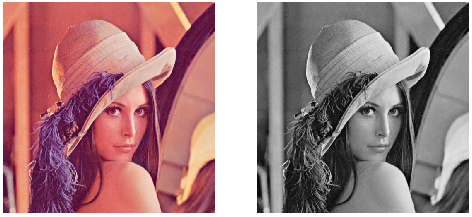
\includegraphics[width=0.46\textwidth]{lenagray2.png}
\caption{Grayscale Conversion}
\label{gray}
\end{figure}
If, in the worst case, some input frames do not have all the $R,\ G,\ B$ values, we simply regard the first channel as its grayscale value.

\subsection{Spatial Smoothing}
The possible bacground noise of original frames could have significant negative effects on accurate motion detection. And thus a 2D spatial smoothing filter is considered to be applied to the frames before applying the temporal derivative filter. Here we tried $3\times3$, $5\times5$ box filters, and $2D$ Gaussian filter with different standard deviation $\sigma$.

\subsection{Temporal Derivation} 
Since the temporal derivatives of each pixel are to be analyzed for large gradients, different temporal derivative filter has different corresponding result. Here we make a comparison between $1st$ and $2nd$ discrete differential as well as $1D$ Gaussian filter with different standard deviation $\sigma$.

\subsection{Threshold Selection}
As shown in Fig \ref{thres}, pixels at different location has different overall behaviours. Those pixels located where no moving objects passed through tend to distribute with in a rather small value range, especially after spatial smoothing. While those pixels contains moving objects tend to have several extreme peaks.

\begin{figure}[thpb]
\centering
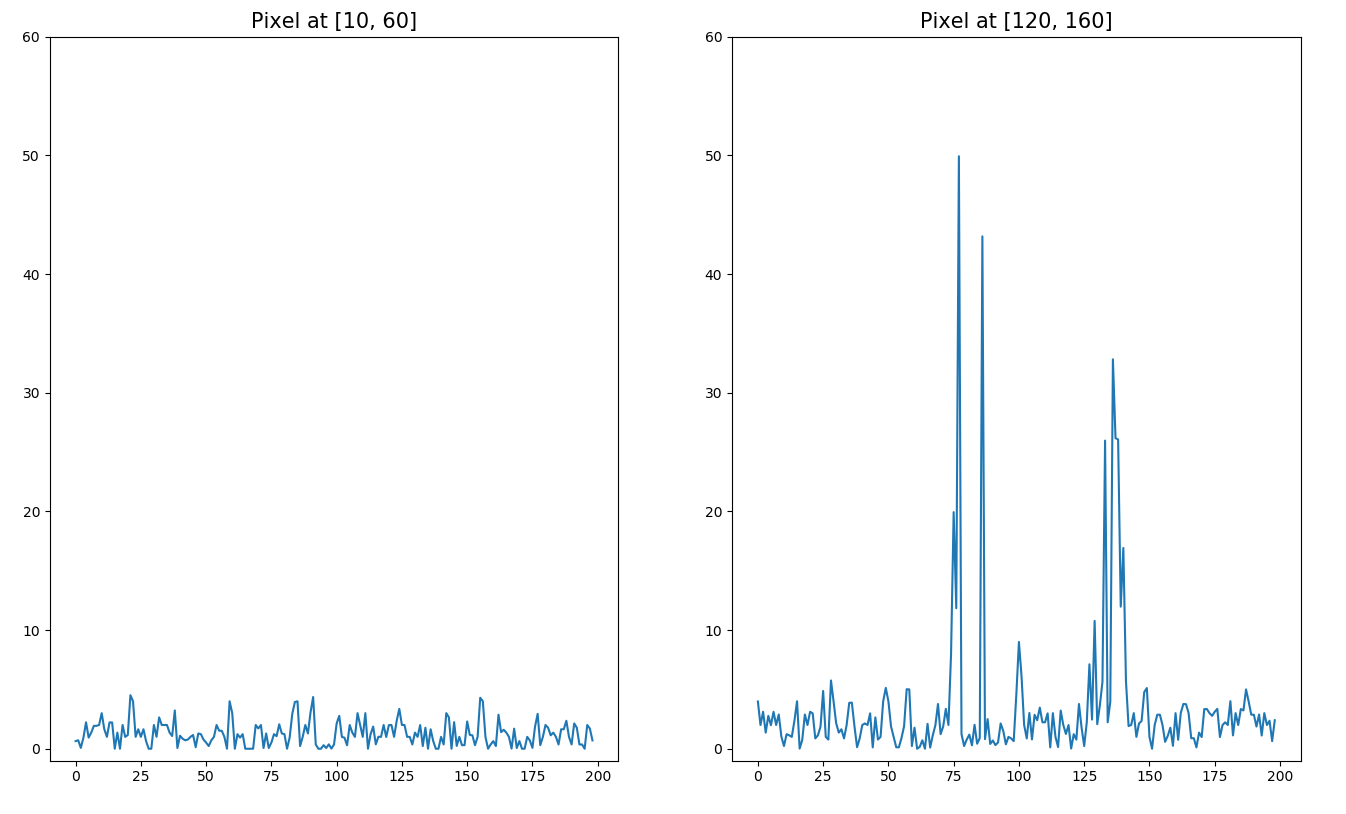
\includegraphics[width=0.46\textwidth]{pixel.png}
\caption{Temporal Derivation of Different Pixels}
\label{thres}
\end{figure}

The threshold selection is of vital importance for accurate motion detection. A threshold which is too high may results in mis-detection of moving objects, while a threshold which is too low can lead to high false alarm rates.

Our threshold selection strategy is based on the assumption that the given frame sequences always contains some percentage of pixels that have no moving objects passing through from start to end. We can then model these pixels as Gaussian zero mean noise based on their standard deviation, and come out with a relatively reasonable overall threshold. 

\subsection{Result Generation}
Once threshold is selected, pixels of each frame can be determined as whether moving or not, and thus we can generate a mask on the original frame to indicate the moving objects.

\begin{equation}  
Mask = \left\{  
     \begin{array}{cc}  
     1, & derivation > threshold\\  
     0, & derivation \leq threshold\\   
     \end{array}  
\right.  
\end{equation}  

%-------------------------------------------------------------------------
\section{EXPERIMENTAL RESULTS}
\subsection{Temporal Derivative Filter}
We use $0.5[-1\ 0\ 1]$ as derivative filter, and use $1D$ Gaussian filter with standard deviation of $\sigma=1, 1.6, 2.5$. After convolved with Gaussian filter, the extreme peaks becomes much smooth, because the overall background noise is reduced. The height of peaks also decreases, which indicates that the mean and standard deviation of each pixel are also reduced. Intensity values of pixels without motion tend to distributed within a smaller range and could be easier to be separated.

\begin{figure}[thpb]
\centering
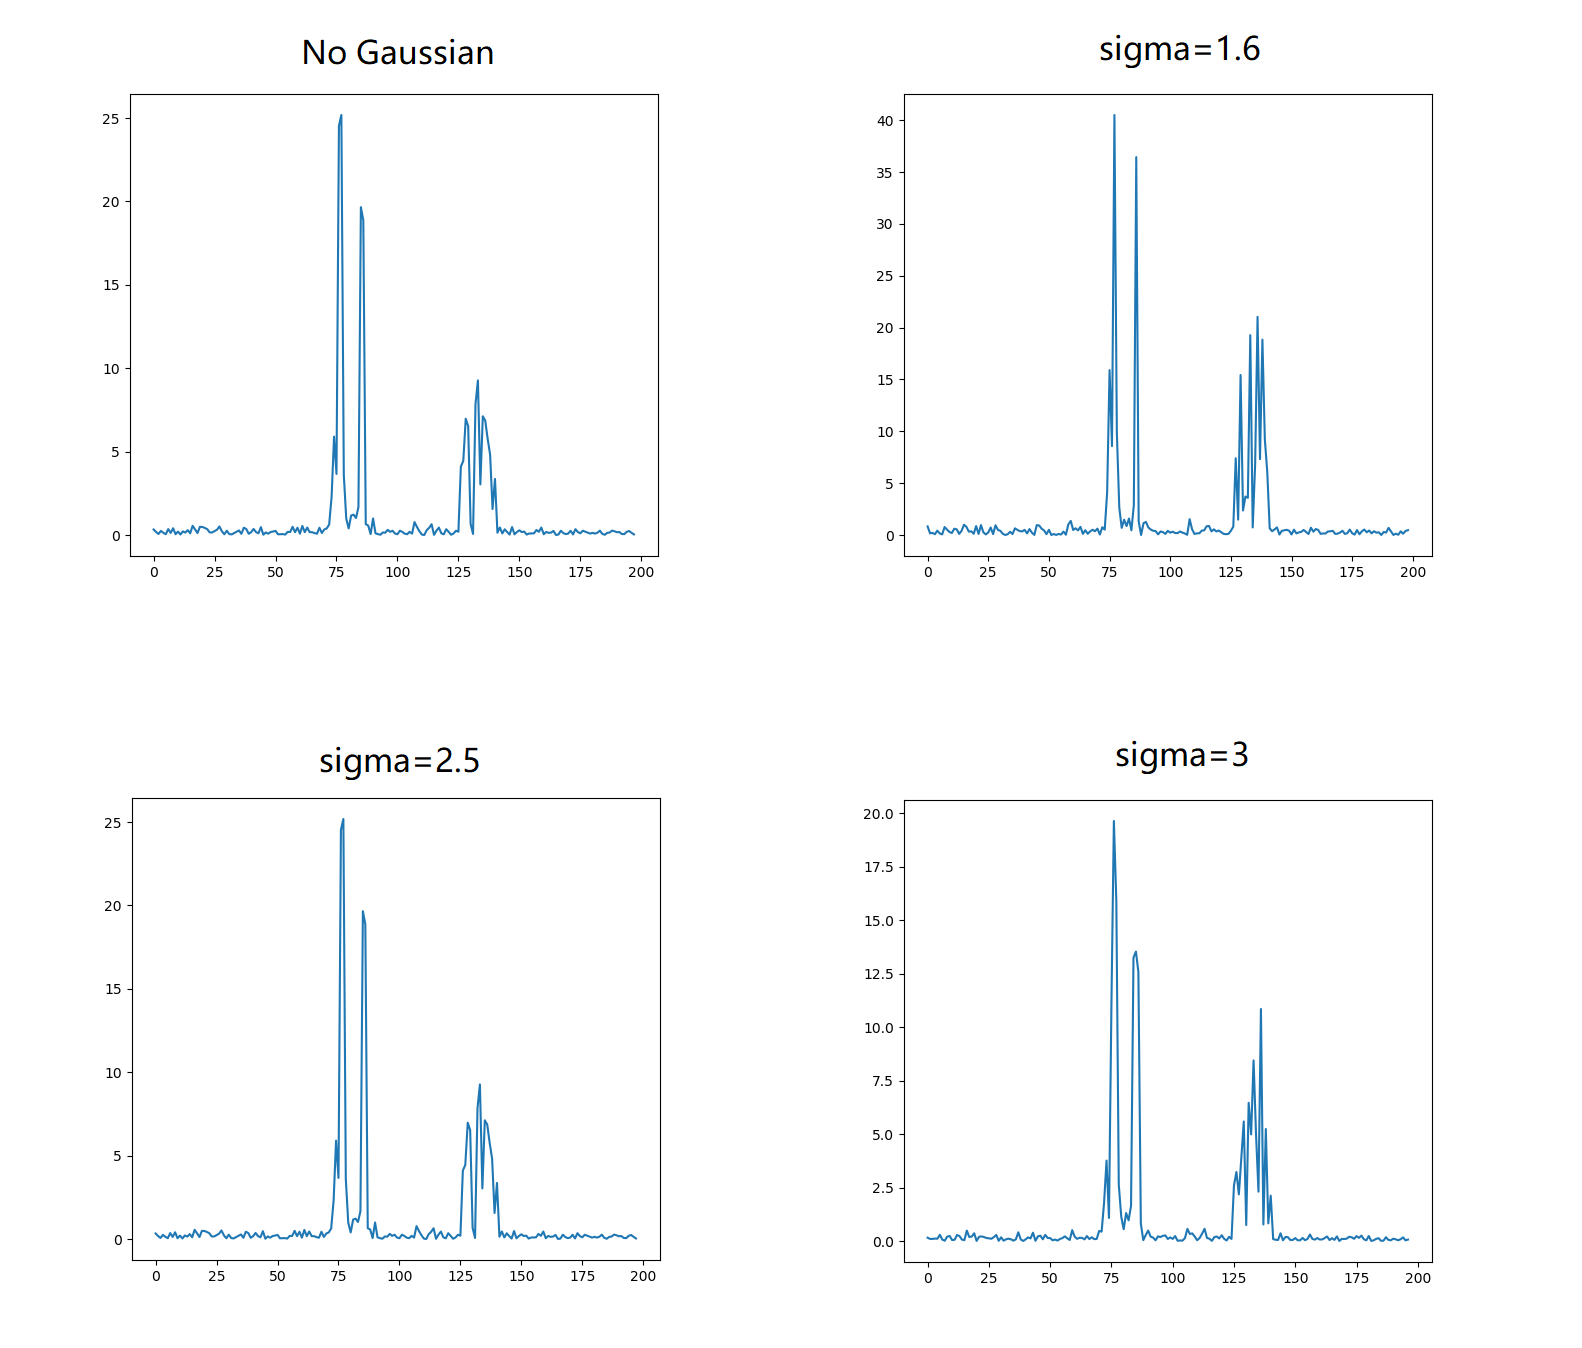
\includegraphics[width=0.4\textwidth]{derivative.png}
\caption{Temporal Derivative Filter}
\label{der} 
\end{figure}

\subsection{Spatial Smoothing Filter}
We utilized four spatial filters for comparison: $3\times3$ Box, $5\times5$ Box, Gaussian $\sigma = 1.4$ and Gaussian $\sigma = 1.8$. A spatial smoothing filter can filter out high frequency noise and also blur frames. We picked one frame from \textit{Office} folder. 

\begin{figure}[thpb]
\centering
\includegraphics[width=0.3\textwidth]{ssf.jpg}
\caption{Original Frame}
\label{ssf} 
\end{figure}

As shown in Fig \ref{dssf}, the background noise is significant before spatial smoothing, and thus the result mask contains several noise spots. As the amount of blur increase, the number of noise point spots decreases and the margins become smooth. Background noise still remains after $3\times3$ box filter, but it almost disappears after $5\times5$ box filter and Gaussian filters. The result is then much more better after spatial smoothing filters as it reduces background noise and separate the moving object. 

However, we should note that though spatial smoothing filter reduces background noise, it also lose details of object. As the amount of blur increase, object tends to `collapse' into a huge pixel, where we cannot separate glasses, face and pleats. 


\begin{figure}[thpb]
\centering
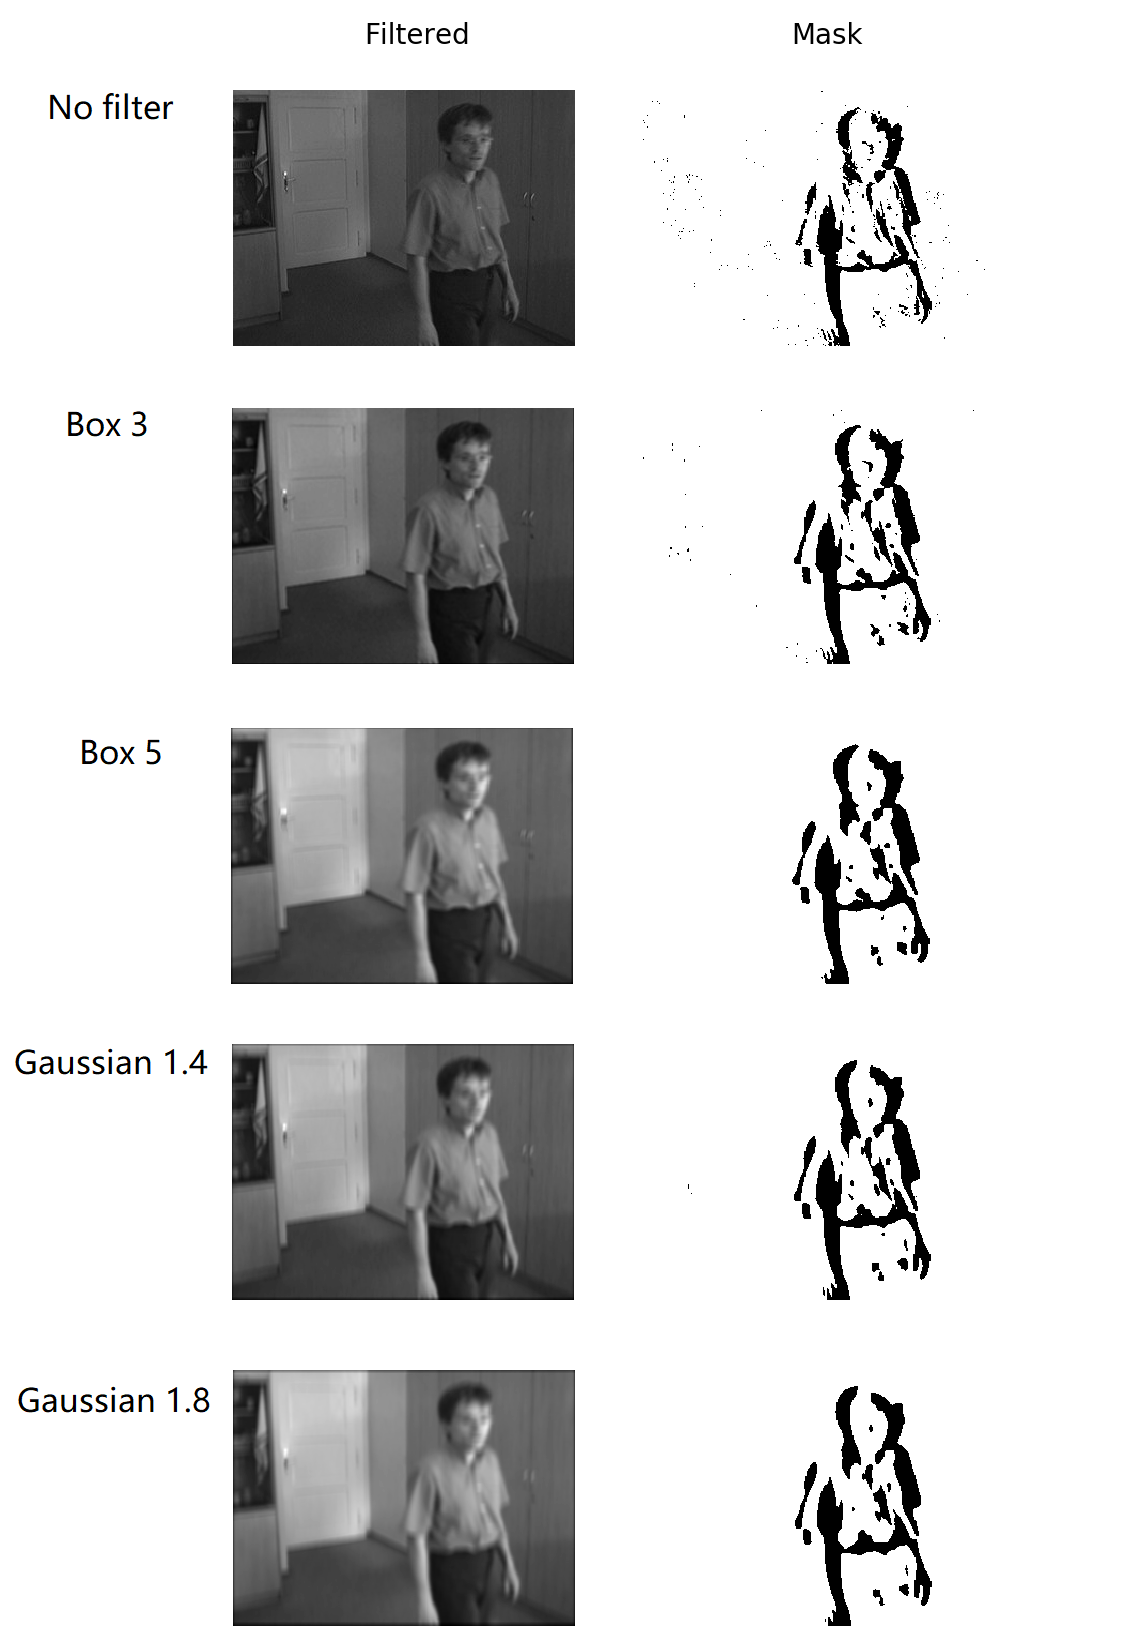
\includegraphics[width=0.46\textwidth]{no.png}
\caption{Different Spatial Smoothing Filters}
\label{dssf}
\end{figure}

\subsection{Threshold Selection}
For each pixel we compute it overall mean and standard deviation, and ascending re-sort them respectively. As assumed that a particular percentage of pixels that contains no moving objects, our threshold selection strategy depends only on the percentage. Once percentage is determined, e.g. $10\%$, the threshold is then determined as $M + 3\Sigma$, where $M$ is the maximum of first $10\%$ mean and $\Sigma$ is the maximum of first $10\%$ standard deviation. Here in Gaussian, less than $1\times 10^{-6}$ samples located outside range $\mu\pm5\sigma$.

As we increase the percentage in Fig \ref{threshold}, the detector is less sensitive to change of intensity values, and the boundaries in mask becomes narrower. We select $10\%$ as our general threshold.

\begin{figure}[thpb]
\centering
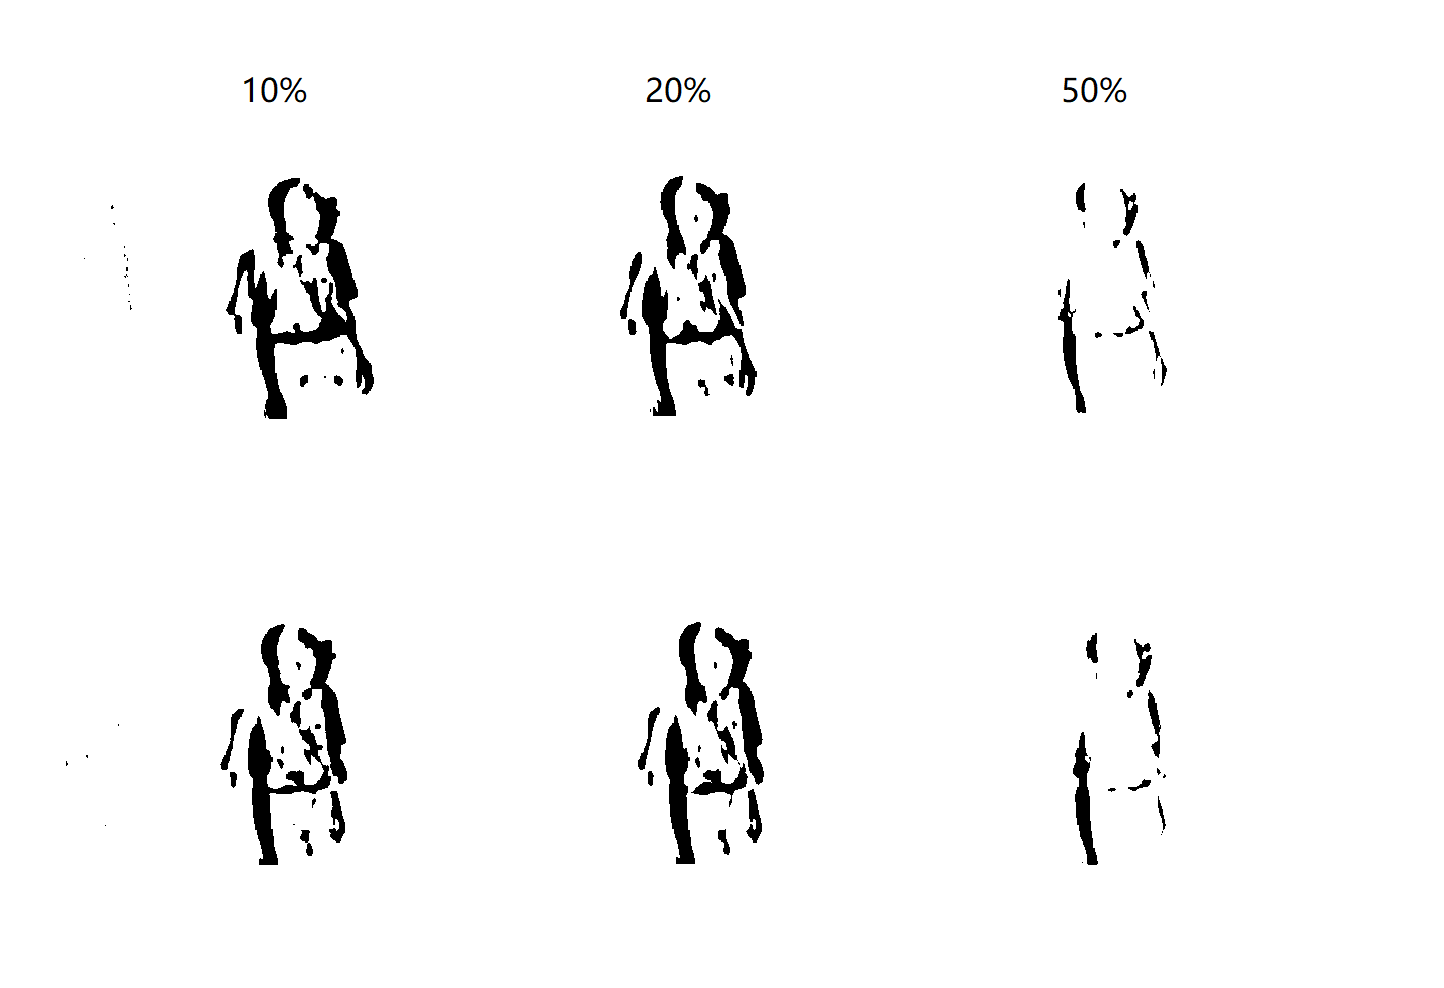
\includegraphics[width=0.5\textwidth]{threshold.png}
\caption{Different Threshold}
\label{threshold}
\end{figure}



\subsection{Limitation}
One of the key limitations of our current motion detection method is that since the motion is detected based on its intensity values, slight changes of light can result in false positive. The frame sequences in Fig \ref{light} demonstrates a mis-detection of light instead of motion.
\begin{figure}[thpb]
\centering
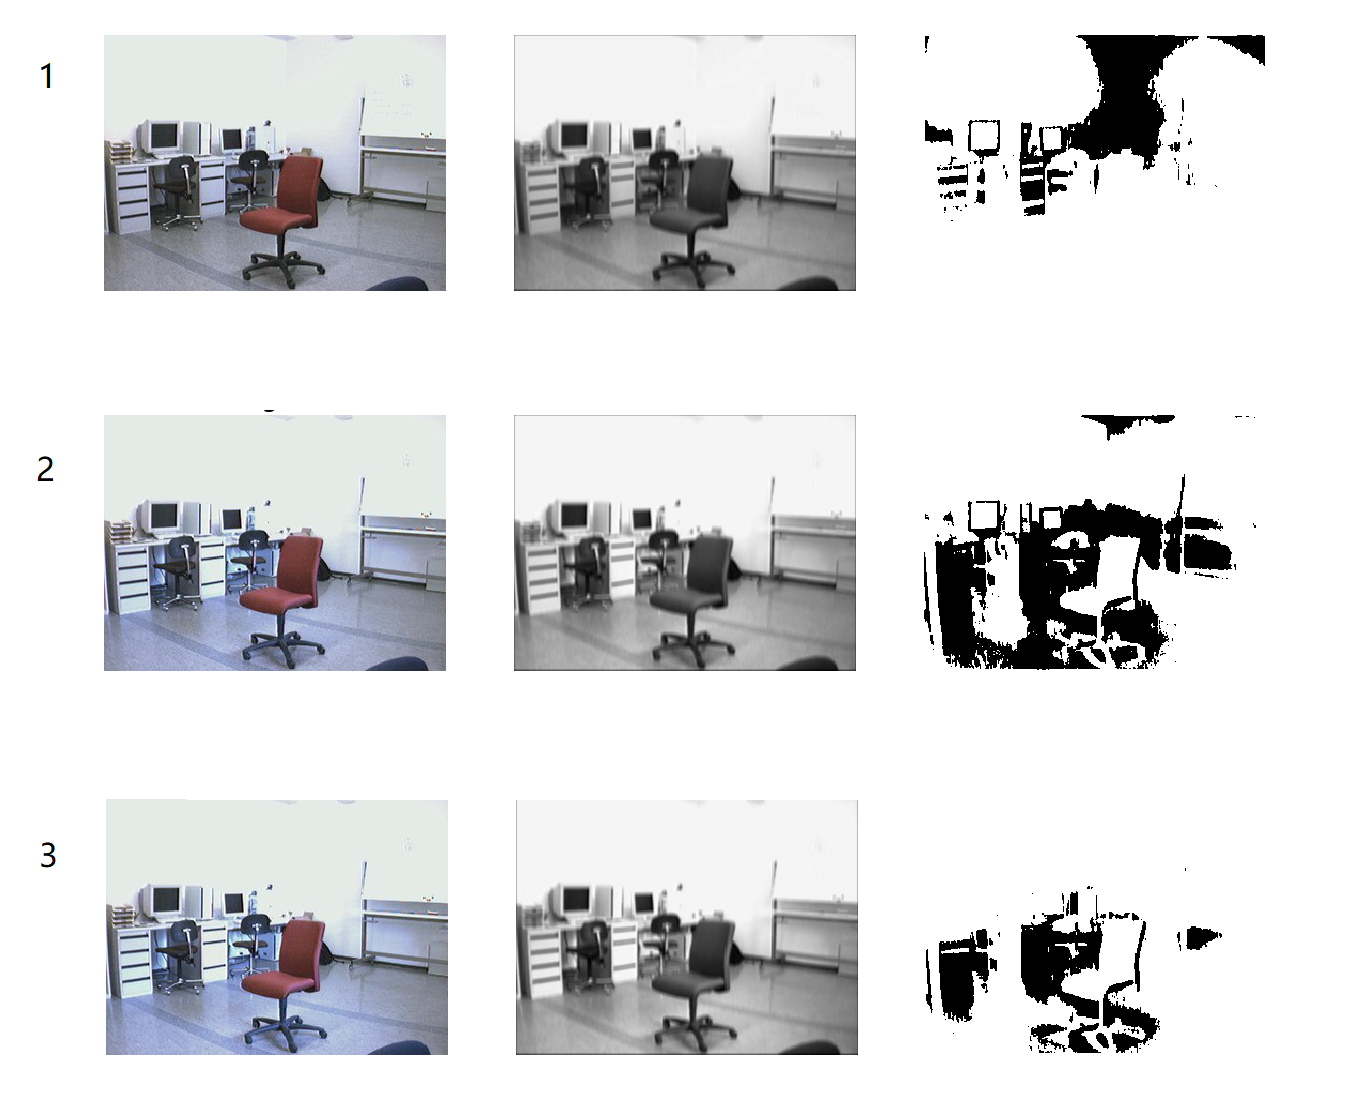
\includegraphics[width=0.46\textwidth]{light.png}
\caption{Light Detection}
\label{light}
\end{figure}

Another weakness of the algorithm is that it tends to capture the motion of object edges but lefts aside in-between. We can always generate masks as shown in Fig \ref{bound}, where the texture of desk even appears inside the human body!

\begin{figure}[thpb]
\centering
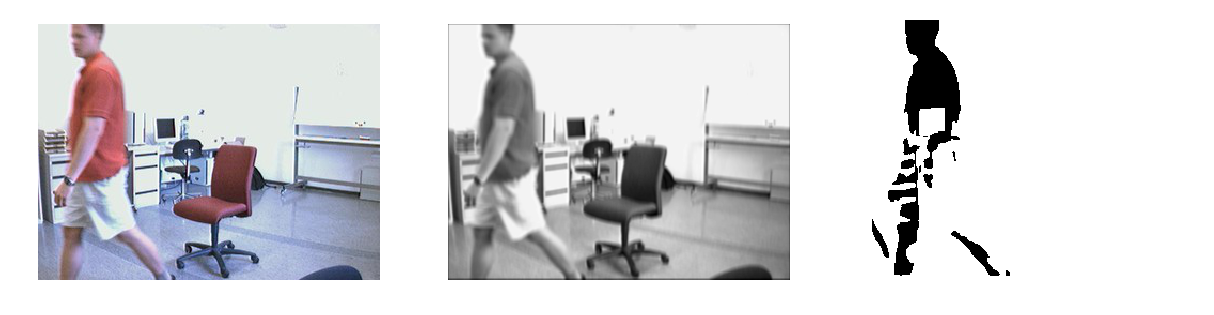
\includegraphics[width=0.46\textwidth]{margin.png}
\caption{Boundaries}
\label{bound}
\end{figure}

%-------------------------------------------------------------------------
\section{CONCLUSION}
Motion detection based on change of the intensity values is a straight forward method and is also efficient. We do not need to consider correlation of different part of moving object and other dynamic factors, which makes the algorithm ease to implement.

The algorithm may be accurate on some simple cases, but it limitation is also significant. If we are to realize more applicable motion detection, more complicated algorithms are to be explored.


\end{document}